%==============================================================================
%== template for LATEX poster =================================================
%==============================================================================
%
%--A0 beamer slide-------------------------------------------------------------
\documentclass[final]{beamer}
\usepackage[orientation=portrait,size=a0,
            scale=1.25         % font scale factor
           ]{beamerposter}

\geometry{
  hmargin=2.5cm, % little modification of margins
}

%
\usepackage[utf8]{inputenc}

\linespread{1.15}
%
%==The poster style============================================================
\usetheme{sharelatex}

%==Title, date and authors of the poster=======================================
\title
%[Super Conference, 1 - 10 July 2013, New York, USA] % Conference
[Machine Learning Final Presentation, January 2019, Beijing]
{ % Poster title
Analysis and Prediction of Cryptocurrency Prices
}

\author{ % Authors
Péter Garamvölgyi\inst{1}, Federico Zaiter\inst{1}
}
\institute
[Tsinghua University] % General University
{
\inst{1} Tsinghua University, Beijing
}
\date{\today}

% added formatting
\setbeamertemplate{caption}[numbered]
\setlength{\parskip}{\baselineskip}



\begin{document}
\begin{frame}[t]
%==============================================================================
\begin{multicols}{3}
%==============================================================================
%==The poster content==========================================================
%==============================================================================

\section{Introduction}

\subsection{Problem overview \& motivation}

Stock market price prediction is a well-established area of study with numerous applications of machine learning models on financial time series \cite{ref1, ref2}. In this work, we evaluate the use of these models for the related problem of cryptocurrency price prediction. The unique characteristics of these time series being non-stationary and volatile introduce challenges. Deep learning models are a potential candidate to tackle these.

\subsection{Data}

For working with Bitcoin price data, there are multiple freely available datasets online. We decided to use Bitstamp's BTC-USD dataset for the period between 1st January 2012 and 11th November 2018. This dataset contains features like the current exchange rate and trading volume. 

One well-known fact about cryptocurrency prices is their significant short- and long-term volatility. To have a stable basis to build on, given recent spikes and dips at the start of the year 2018, we chose to evaluate our models on the time period between 1st January 2016 and 20th October 2017.

\vskip1ex
\begin{figure}
\centering
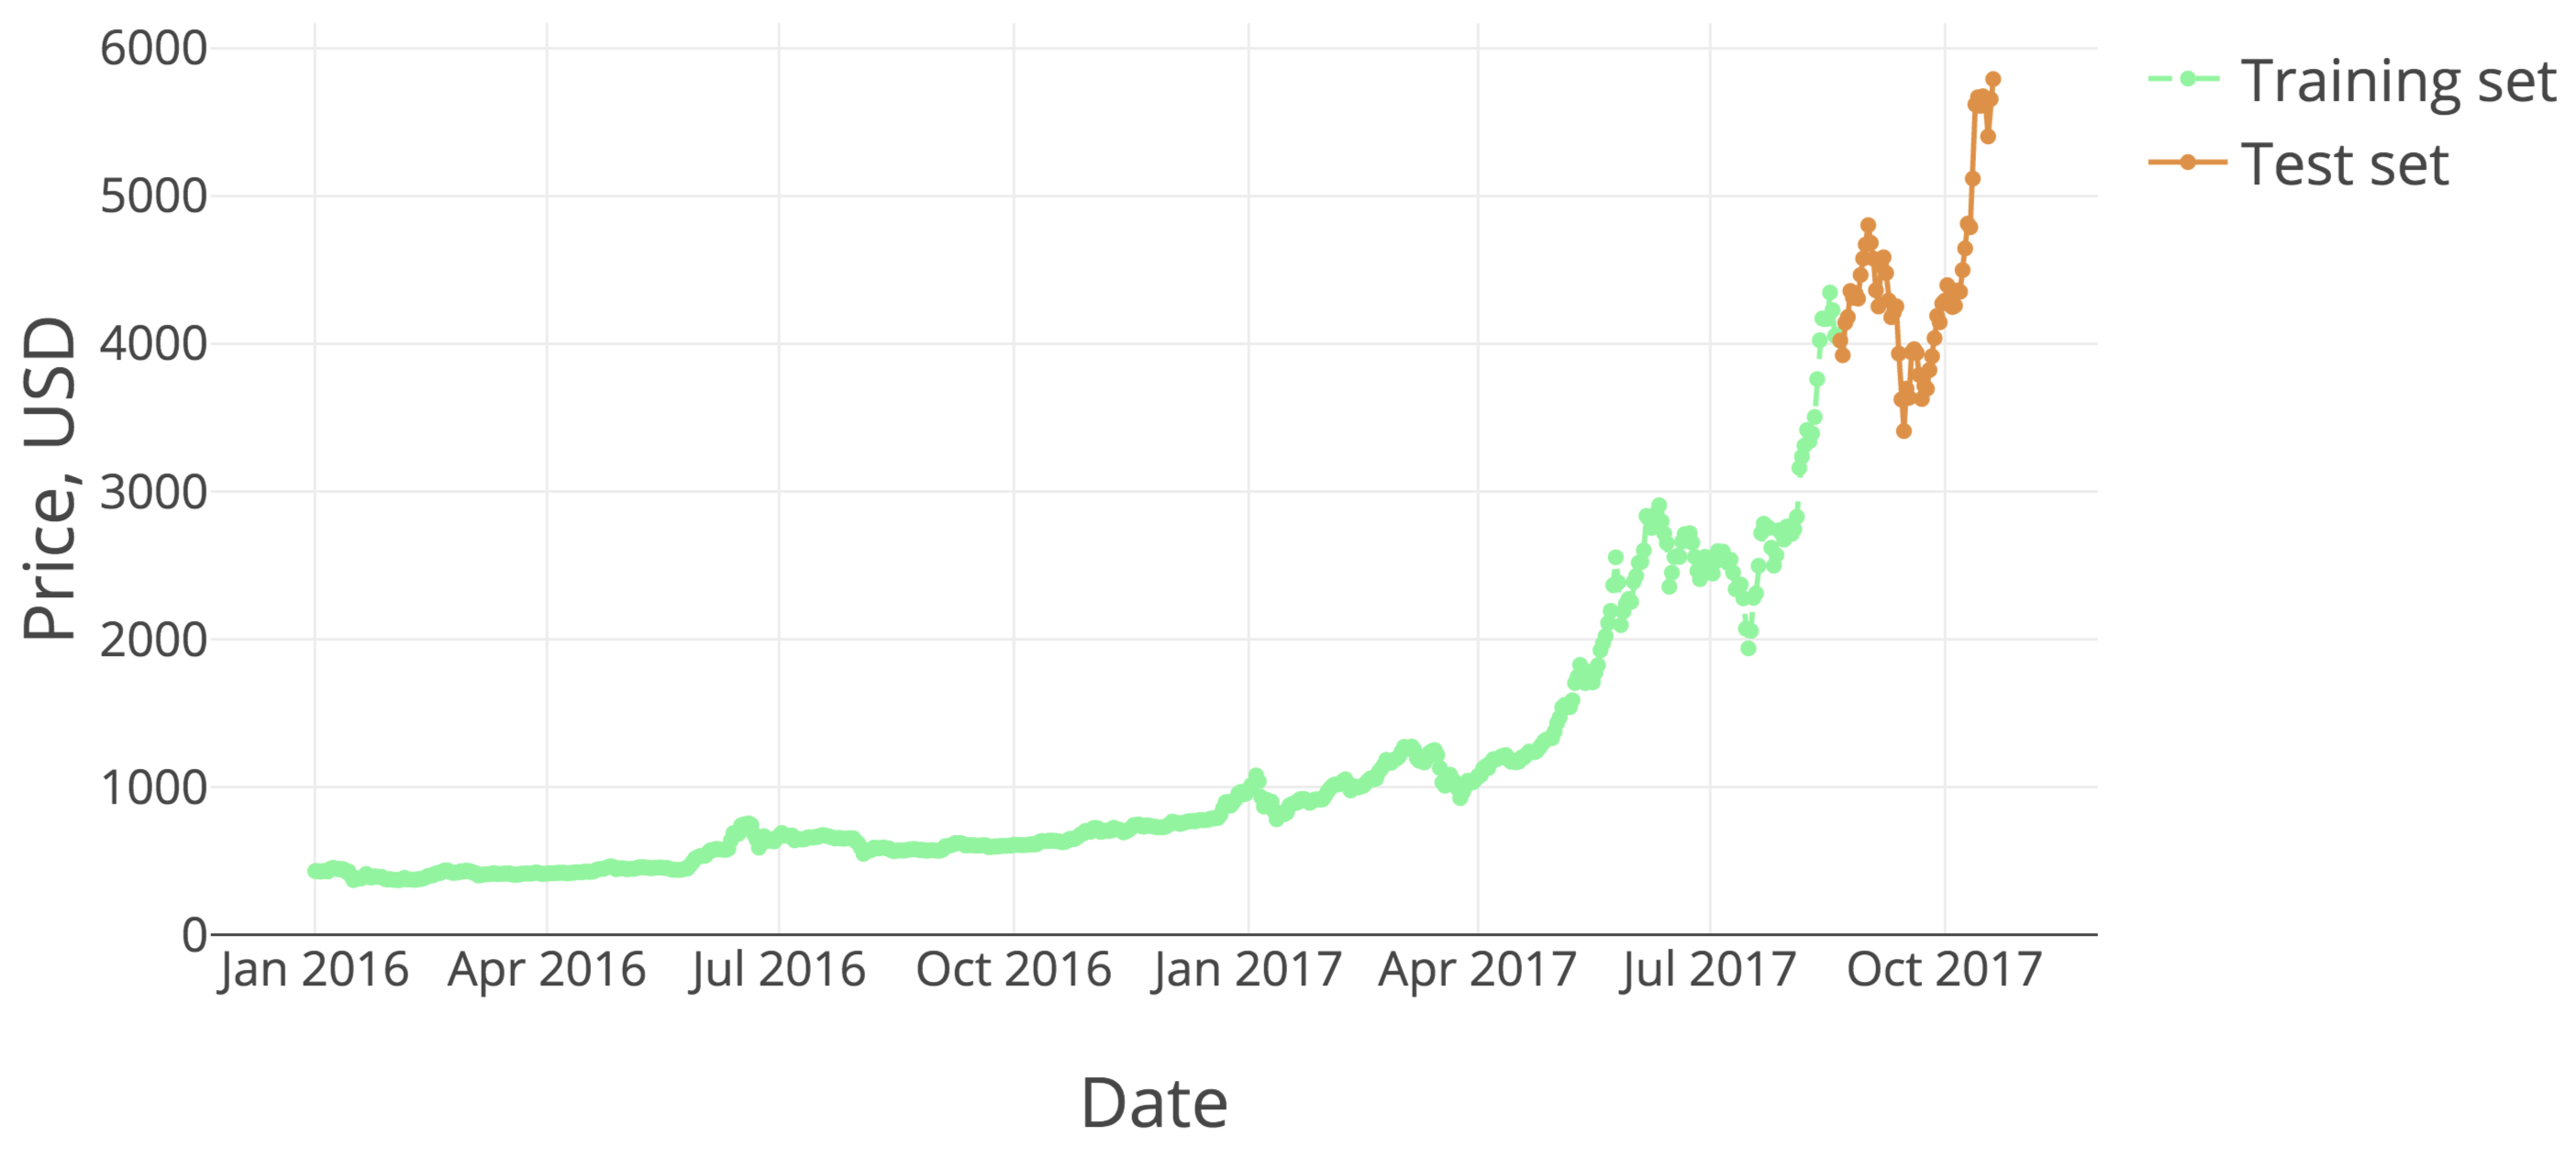
\includegraphics[width=0.99\columnwidth]{images/dataset.png}
\caption{Bitcoin price dataset}
\label{fig:dataset}
\end{figure}
%\vskip2ex

\subsection{Preprocessing}
From this dataset, we only keep the price data daily aggregated, turning this into a univariate time series modeling and forecasting problem. For separating the data into training and test sets, we tried two approaches.

\begin{enumerate}
    \item Choose a date and use it to cut the dataset into two (figure \ref{fig:dataset}). This is a common approach; however, the significant differences during different periods in our dataset might have a negative impact on the generalization ability of this approach.
    \item Cut the original dataset into \emph{chunks} of equal duration and then separate each of these into training and test sets. This approach will result in a more representative collection of data points. 
\end{enumerate}

For LSTM, we do further preprocessing by generating sliding windows of training data input and expected results as well as normalizing the data. 


\section{Single-step prediction}

First, let us discuss the problem of single-step prediction. In this scenario, we are given a time window of the last $n$ price values. Our goal is to predict the price in the next time step immediately after this window. An example is predicting tomorrow's price based on the last 7 days.

\vspace{-1.2em}
$$single\textnormal{-}pred(a_1, a_2, ..., a_n) \approx a_{n+1}$$

Our baseline for single-step prediction is a lag predictor: We simply assume that the price has not changed since the last day. 

\vspace{-1.2em}
$$single\textnormal{-}pred_{baseline}(a_1, a_2, ..., a_n) = a_n$$

We tried two other models for single-step prediction: ARIMA and LSTM \cite{ref3}. ARIMA is a statistical model often used for stationary time series. LSTM, on the other hand, is a type of RNN often used for diverse time series applications.

For evaluation, we use the RMSE metric computed on the test set after training. The RMSE of the different models used do not differ significantly at \$160. This suggests that LSTM approximated the baseline but was unable to learn a better prediction based on the limited data available. Also given the simplicity of the prediction at hand, it would be hard to beat a simple solution.


\section{Multi-step prediction}

In this section, we will present our results for multi-step prediction. In this scenario, we are given a time window (called \emph{look-back}) of the last $n$ price values. Our goal is to predict the price values for the next $m$ steps immediately after this window (called \emph{look-ahead}). An example would be predicting the next seven days' prices based on data from the past three weeks.

\vspace{-1.2em}
$$multi\textnormal{-}pred(a_1, a_2, ..., a_n) \approx (a_{n+1}, a_{n+2}, ..., a_{n+m})$$

For choosing the baseline for multi-step prediction, we evaluated three models: simple linear regression, SVM regression \cite{ref4} with radial basis function, and ARIMA, all of them calculated on a single look-back window per prediction. Figure \ref{fig:multi-naive} illustrates some example predictions of these three models; ARIMA delivered the best results during our evaluation, so we chose it as our baseline. As uncertainty grows with every step in multi-step prediction, the corresponding RMSE values are significantly higher than the single-step ones (figure \ref{fig:multi-rmse}). 

\vskip1ex
\begin{figure}
\centering
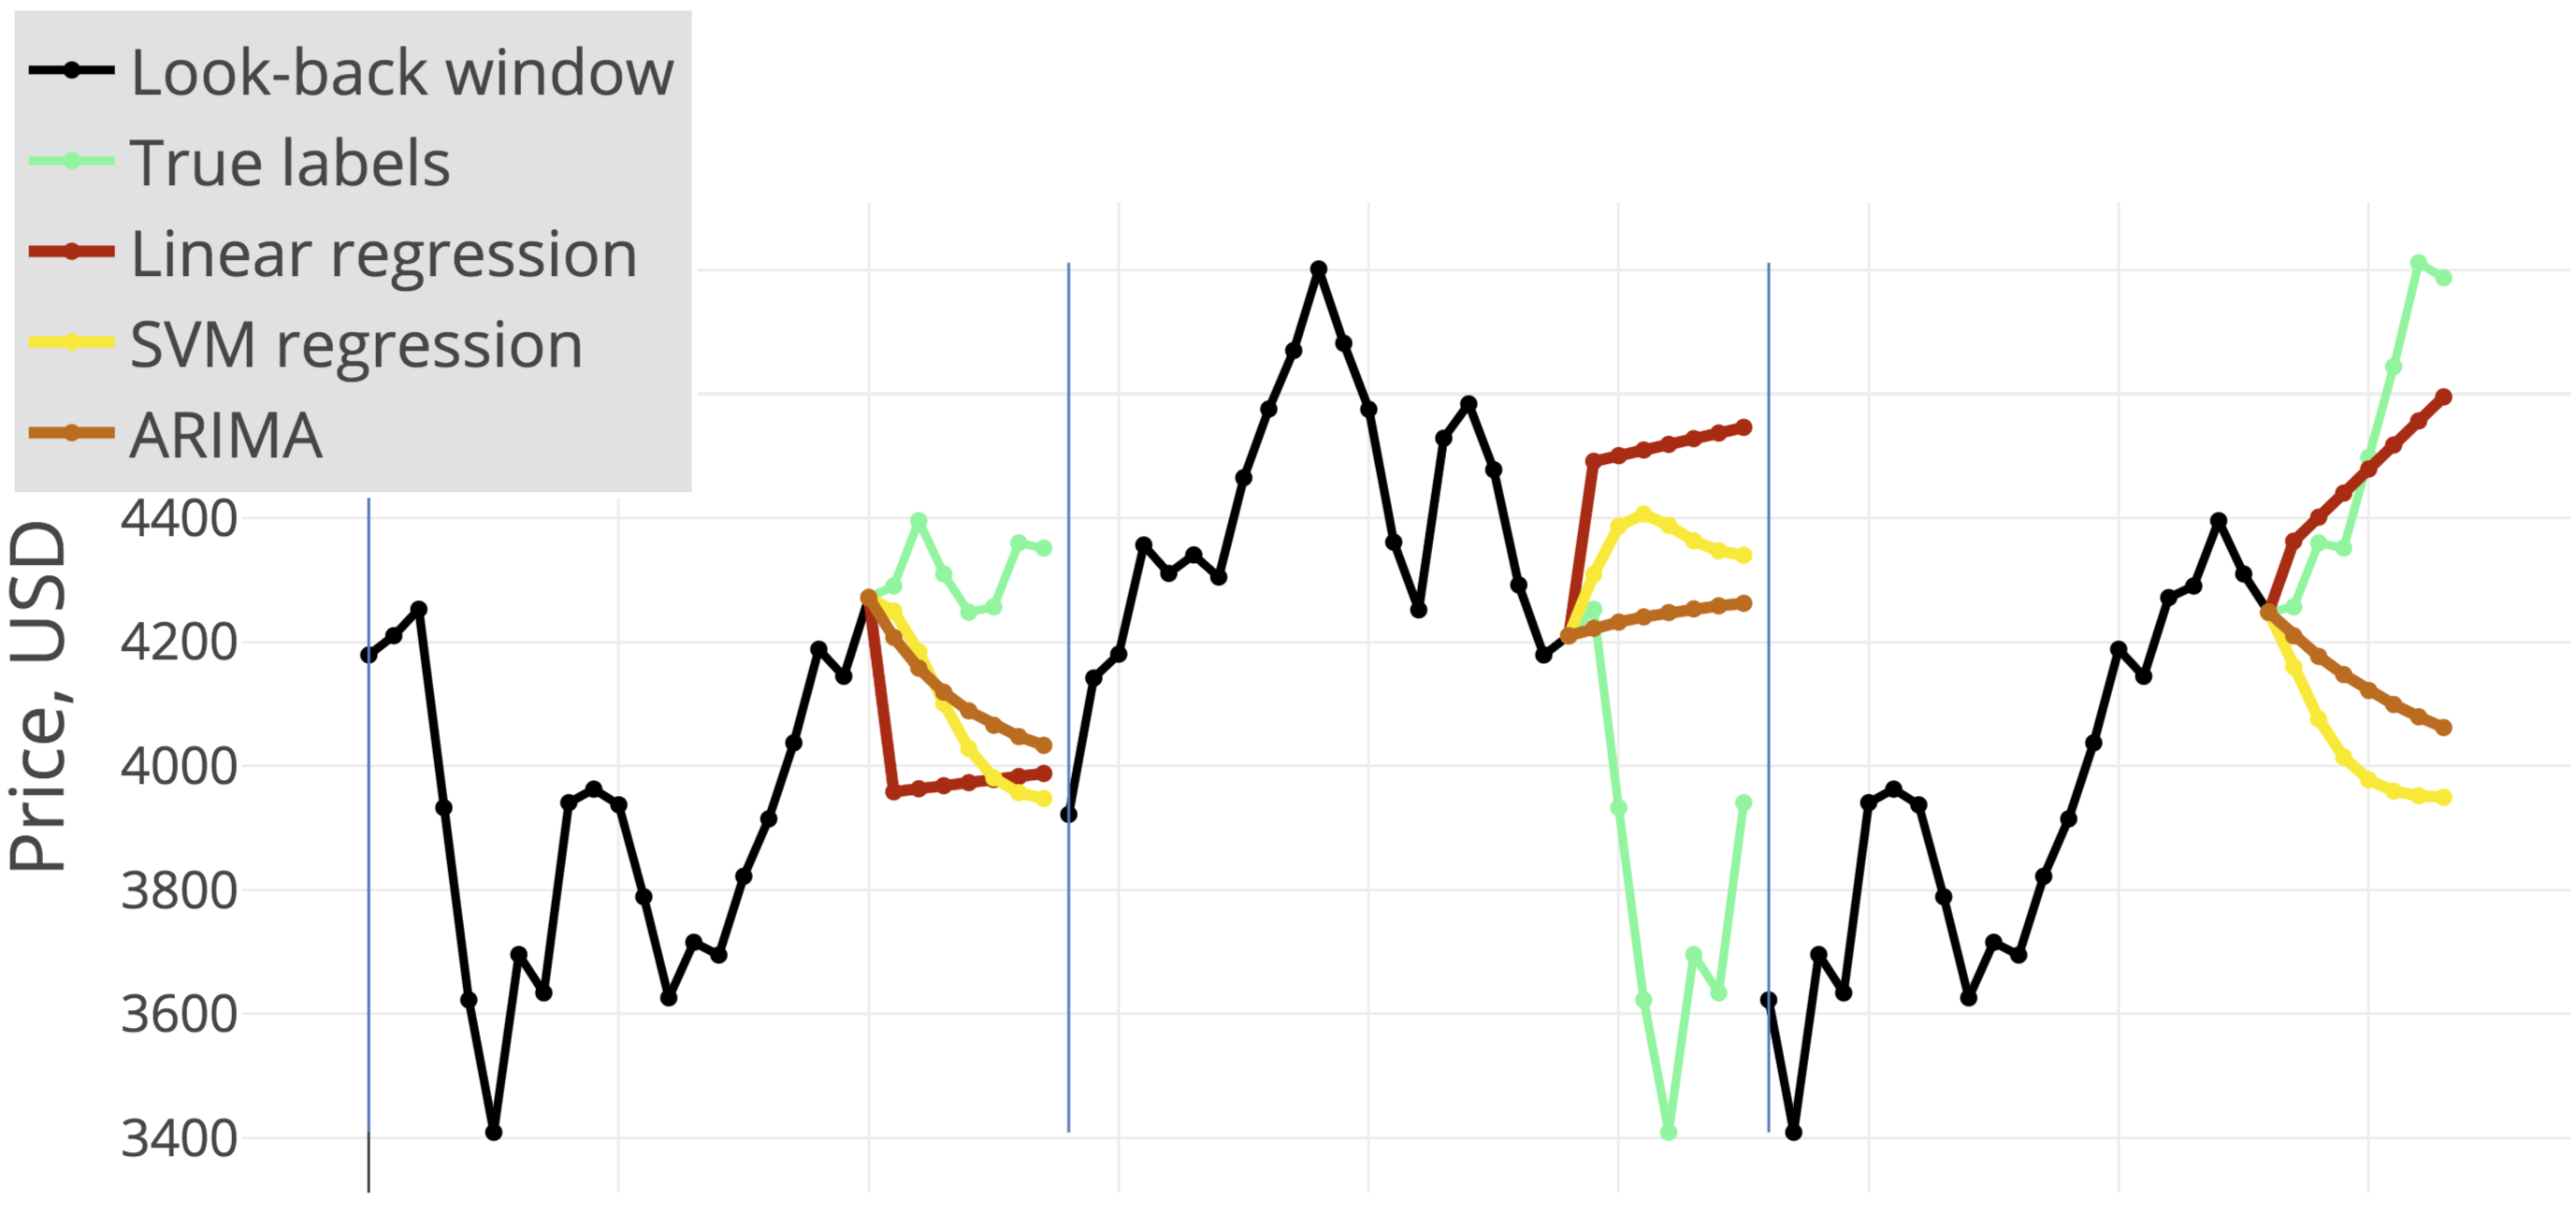
\includegraphics[width=0.99\columnwidth]{images/multi-naive.png}
\caption{Baseline example predictions}
\label{fig:multi-naive}
\end{figure}
%\vskip2ex

Our deep learning model for multi-step prediction is a deep LSTM network. The inputs are the look-back windows, while the outputs are the look-ahead windows.

Figure \ref{fig:multi-lstm} shows example predictions of our trained model.

\vskip1ex
\begin{figure}
\centering
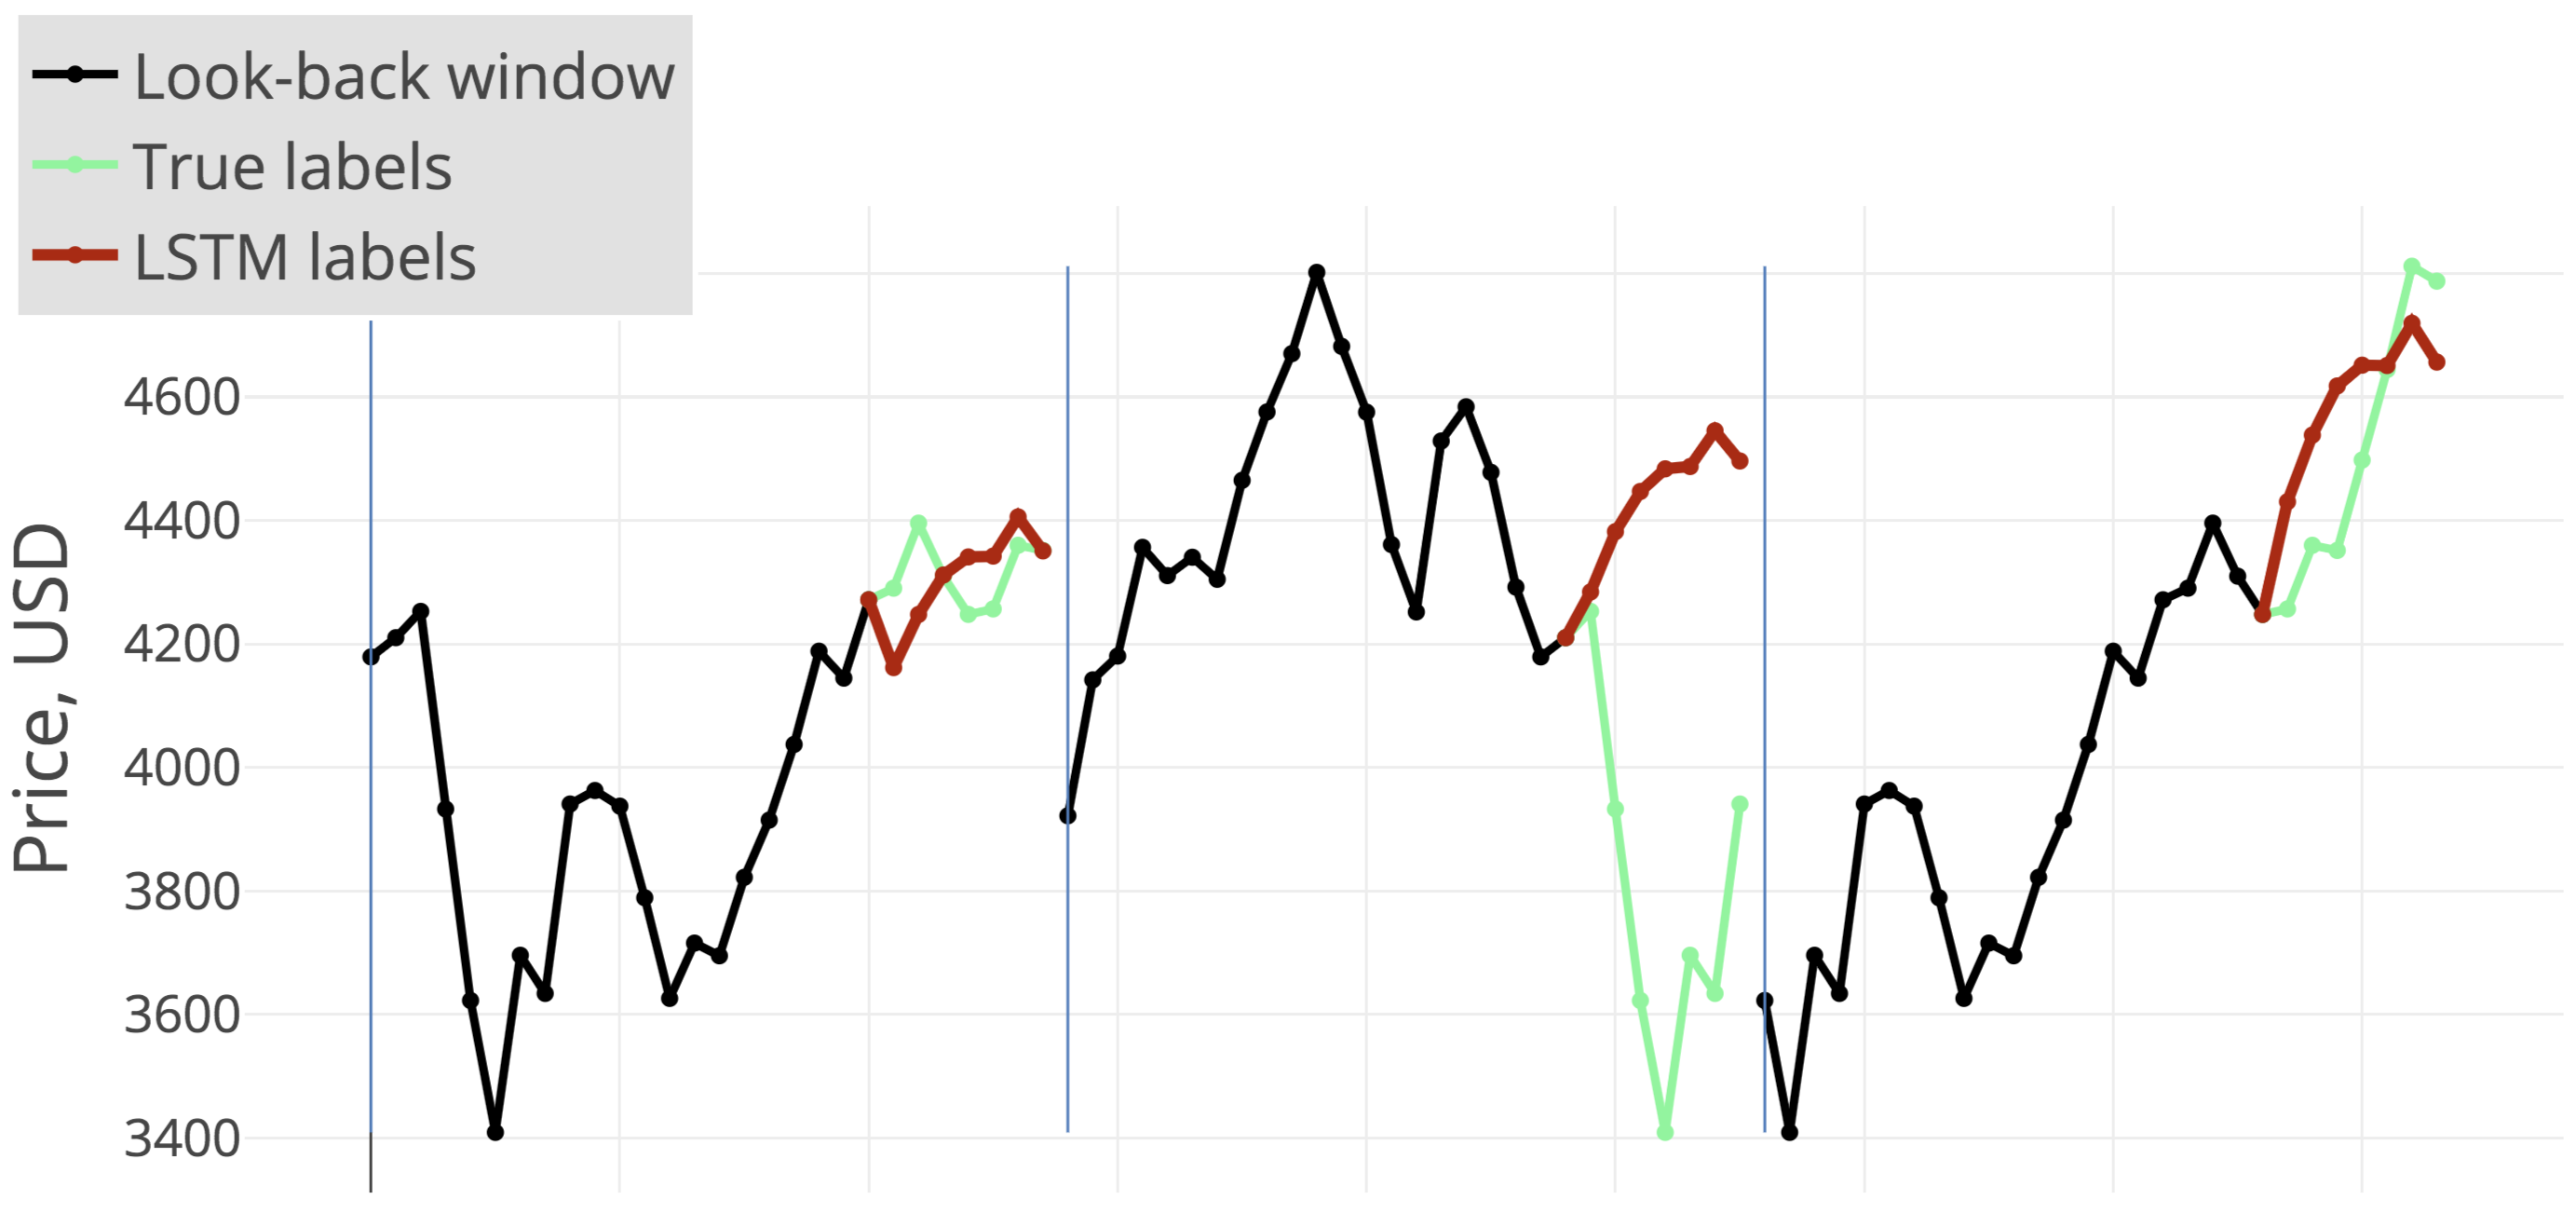
\includegraphics[width=0.99\columnwidth]{images/multi-lstm.png}
\caption{Example predictions using LSTM}
\label{fig:multi-lstm}
\end{figure}
%\vskip2ex

By using LSTM, we achieved a small but significant (about 9\%) improvement in overall prediction error on our test data. While these results rely heavily on the actual series being used, the results suggest that LSMT models can learn some complex changes automatically and thus outperform simple models.

\vskip1ex
\begin{figure}
\centering

\includegraphics[width=0.5\columnwidth]{images/LSTM.png}
\caption{DNN Model}
\label{fig:lstm-model}
\end{figure}
%\vskip2ex

\vskip1ex
\begin{figure}
\centering
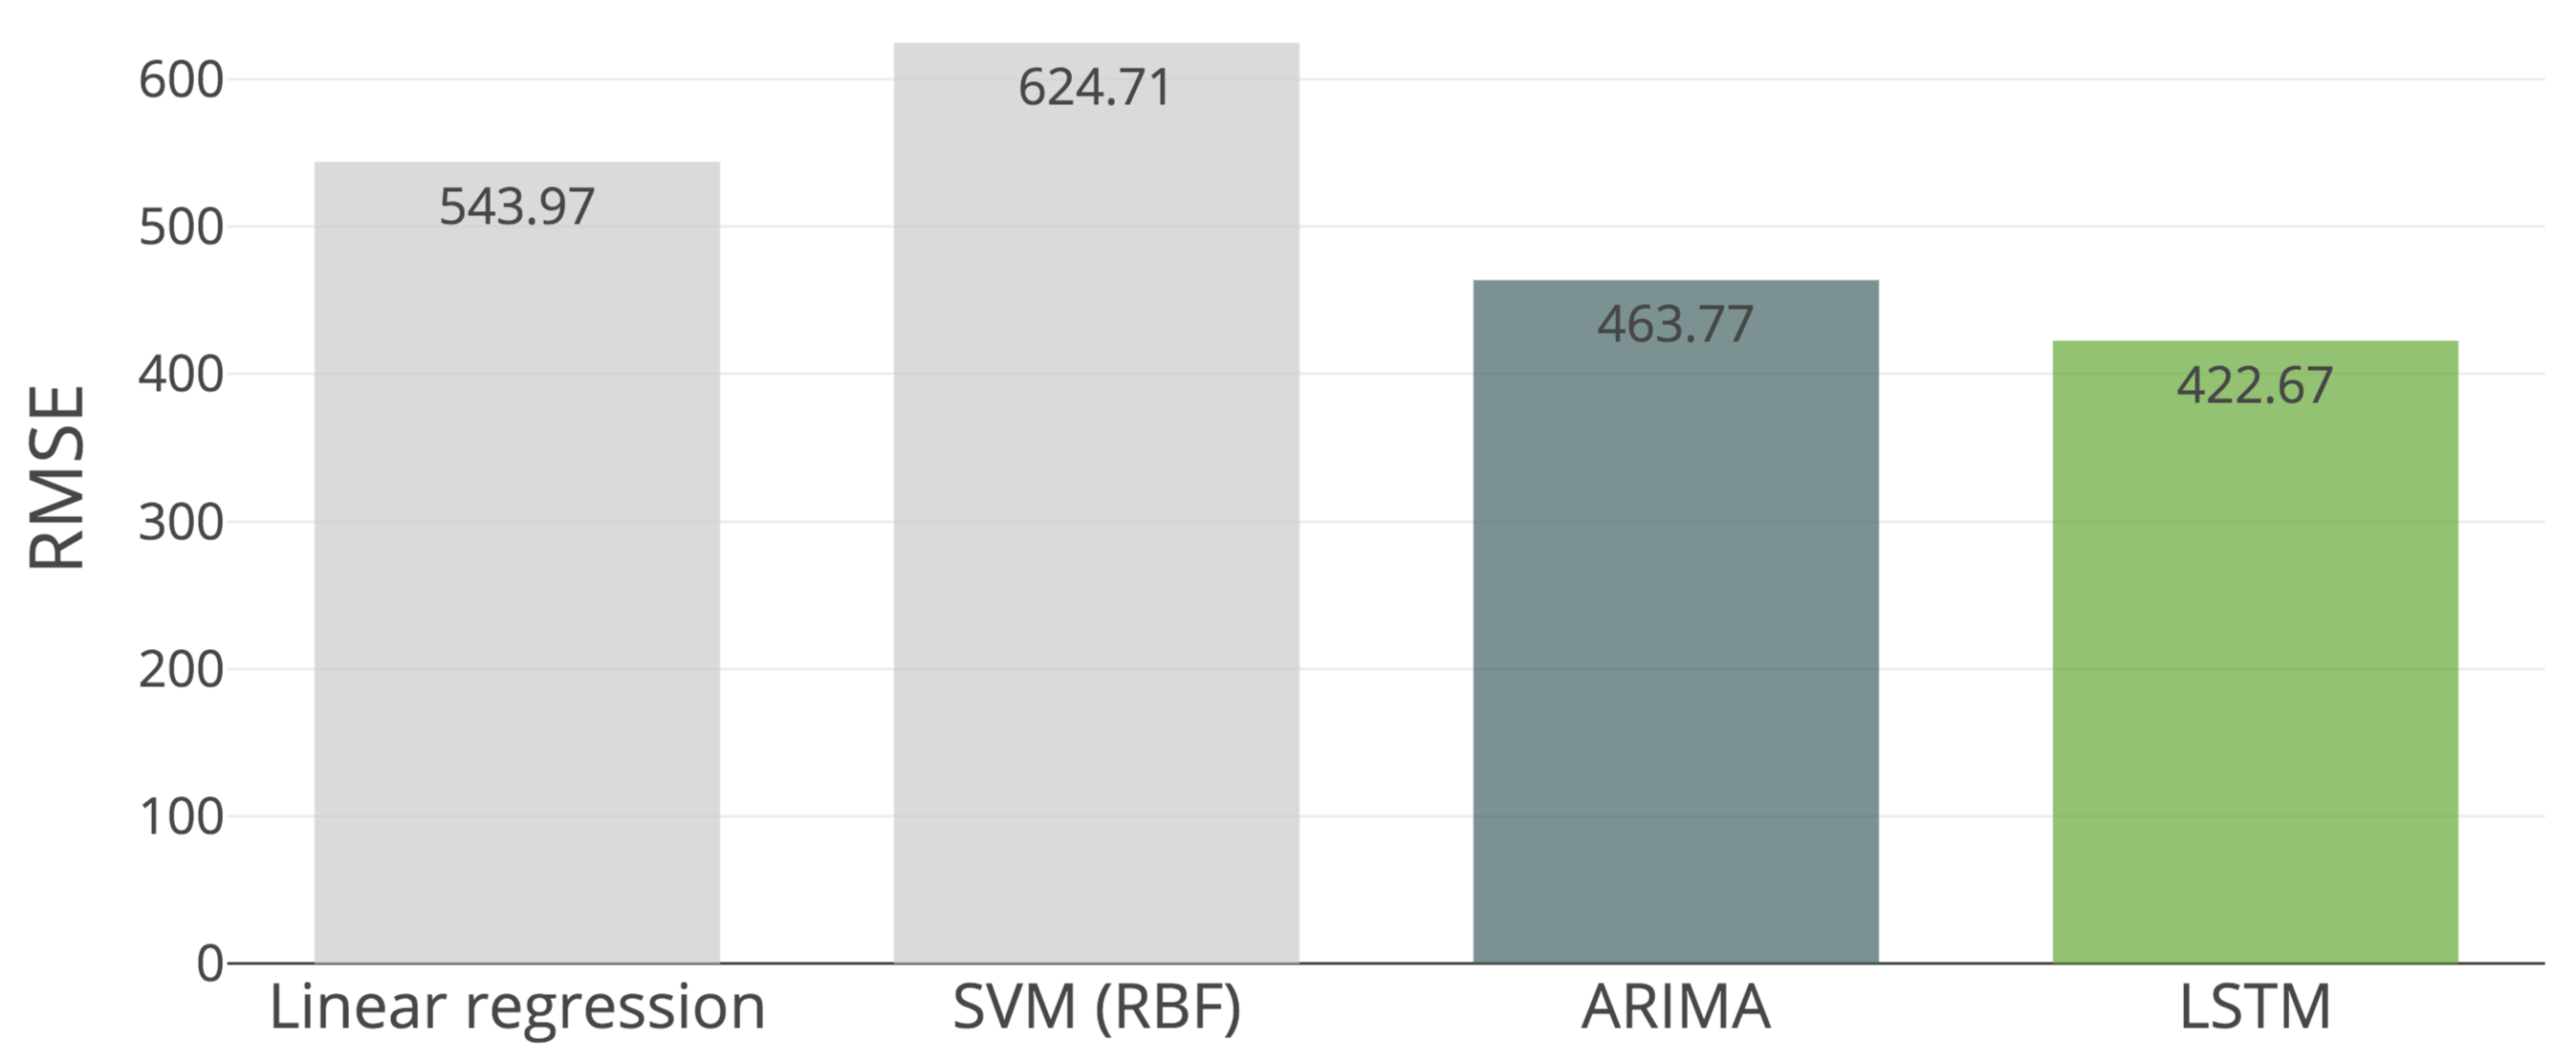
\includegraphics[width=0.99\columnwidth]{images/multi-rmse.png}
\caption{Comparison of prediction errors (RMSE)}
\label{fig:multi-rmse}
\end{figure}
%\vskip2ex


\section{Summary and conclusions}

We evaluated the use of LSTM for both single-step and multi-step time-series forecasting. For single-step prediction, using machine learning models offered no improvement compared to our simple baseline. For multi-step prediction, however, we achieved a \textasciitilde9\% improvement in prediction accuracy with LSTM compared to our best baseline ARIMA.

The results above suggest that the application of deep learning models for price prediction and other time series forecasting tasks is a promising area. Possible future directions for research include a more thorough evaluation of models, hyper-parameter tuning, incorporating more features into the models, and trying the same approaches on other datasets.


%==============================================================================
%==End of content==============================================================
%==============================================================================

%--References------------------------------------------------------------------

\subsection{References}

\begin{thebibliography}{99}

\bibitem{ref1} Ariyo, Adebiyi Ariyo et al. (2014). Stock Price Prediction Using the ARIMA Model. 2014 UKSim-AMSS 16th International Conference on Computer Modelling and Simulation, 106-112.

\bibitem{ref2} Chen, Kai et al. (2015). A LSTM-based method for stock returns prediction: A case study of China stock market. 2015 IEEE International Conference on Big Data (Big Data), 2823-2824.

\bibitem{ref3} Hochreiter, S., \& Schmidhuber, J. (1997). Long Short-Term Memory. Neural Computation, 9, 1735-1780.

\bibitem{ref4} Drucker, H., Burges, C.J., Kaufman, L., Smola, A.J., \& Vapnik, V. (1996). Support Vector Regression Machines. NIPS.

\end{thebibliography}
%--End of references-----------------------------------------------------------

\end{multicols}

%==============================================================================
\end{frame}
\end{document}

